73. Если $f(x)$ является нечётной функцией, то  $f(x)=\begin{cases}-\cfrac{2}{x^2},\ x<0,\\ \cfrac{2}{x^2},\ x>0.\end{cases}$
$$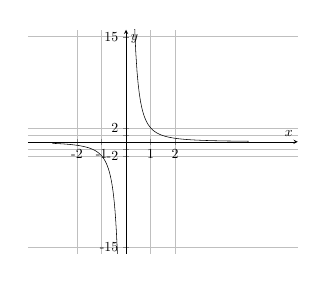
\begin{tikzpicture}[scale=0.5]
\begin{axis}[
    axis lines = middle,
    grid=major,
    legend pos={south west},
    xlabel = {$x$},
    %xlabel style={below right},
    ylabel = {$y$},
    ymin=-16,
    ymax=16,
    xmin=-4,
    xmax=7,
    xtick={-2,-1,1,2},
    xticklabels={-2,-1,1,2},
    ytick={-15,-2,-1,1,2,15},
    yticklabels={-15,-2,$ $,$ $,2,15},
                  ]
	\addplot[domain=-3:-0.1, samples=100, color=black] {-2/(x*x)};
    \addplot[domain=0.1:5, samples=100, color=black] {2/(x*x)};
        %\addplot[domain=2.01:6, samples=100, color=black] {2/(2-x)};
   % \addplot[domain=-3:3, samples=100, color=black] {-x};
     %\addlegendentry{$\text{Рис. 1}$};
\end{axis}
\end{tikzpicture}$$
